\label{unit0}
%Introduction which gives an in-depth description of what MultiSeq does
%Perhaps we could take this out of Elijah's paper


\section{Introduction}



MultiSeq 
(shown in Fig.~\ref{fullDisplay}) 
is a unified bioinformatics analysis environment that allows one to
organize, display, and analyze both sequence and structure data for
proteins and nucleic acids. Special emphasis is placed on analyzing the
data within the framework of evolutionary biology.
MultiSeq was created to allow biomedical researchers to study the
evolutionary changes in sequence and structure of proteins across all
three domains of life, from bacteria to humans.  The comparative
sequence and structure metrics, and analysis tools introduced in the
\begin{figure}[here]
 \centerline{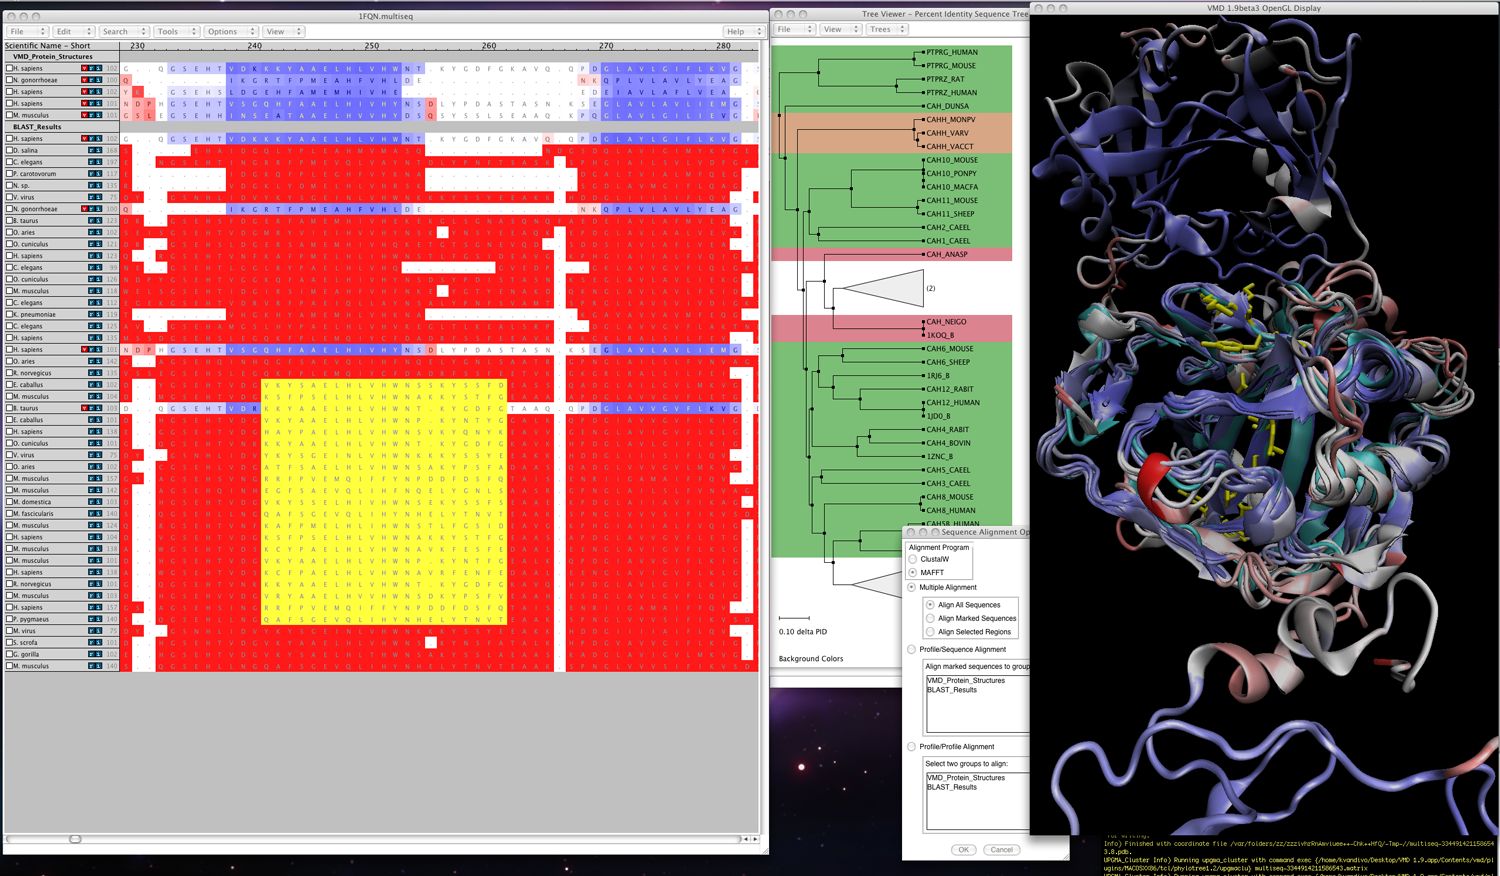
\includegraphics [width=5in]{./pictures/screenShot20110307.png}}
 \caption{MultiSeq In VMD}
\label{fullDisplay}
\end{figure}
article by O'Donoghue and Luthey-Schulten~\footnote {P.
O'Donoghue and Z. Luthey-Schulten. ``Evolution of Structure in
Aminoacyl-tRNA Synthetases''  MMBR, 67(4):550-73.  December, 2003. }
are part of MultiSeq.   In particular,  the Luthey-Schulten
group has included a structure-based measure of
homology \begin{math} Q_H \end{math} (see Appendix B), that takes into
account the effect of insertions and deletions and has been shown to
produce accurate structure-based phylogenetic trees.  The STAMP
structural alignment algorithm, kindly provided by our colleagues
Russell and Barton, is included~\footnote {R.B.
Russell and G.J. Barton. ``Multiple protein sequence alignment from
tertiary structure comparison: assignment of global and residue
confidence levels.''  Proteins: Struct. Func. Genet., 14:309-323.  1992.
}.  
%We plan to offer biomedical researchers a tool to examine the
%changes in protein structure in the correct statistical framework.  
As a result, Multiple Alignment is an invaluable tool for relating
protein structure to its function or misfunction.

In any publication of scientific results based completely or in part on
the use of MultiSeq, please reference:

Elijah Roberts, John Eargle, Dan Wright, and Zaida Luthey-Schulten.
MultiSeq: Unifying sequence and structure data for evolutionary
analysis.  BMC Bioinformatics, 2006, 7:382.


\subsection{Installation}
MultiSeq is part of the standard VMD release.  You can download VMD
from \texttt{http://www.ks.uiuc.edu/Research/VMD/}.  Although BLAST is
not necessary for the overall function of MultiSeq, it is highly
recommended to have BLAST installed locally (i.e. accessible through
file browsing on your local computer).  See
\texttt{http://www.scs.illinois.edu/\~{}schulten/multiseq/} for links to
tutorials with additional information on BLAST installation.

ClustalW is the default sequence alignment tool and is packaged with
MultiSeq.  However, MAFFT (available from
\texttt{http://mafft.cbrc.jp/alignment/software/}) can be used for doing
sequence alignment if it is installed on your computer system.  (MAFFT
version 6.811 has been tested.  Newer versions are expected to work as
well and should be used if possible.)

Paths to all locally installed software and databases are set via the
\textsf{File} | \textsf{Preferences} menu in the MultiSeq window.  The
\textsf{Preferences} menu has a `Metadata' tab and a `Software' tab.
The `Software' tab is where file paths can be provided.

MultiSeq uses a collection of databases that need to be downloaded to
your computer system.  The first time you run MultiSeq you
will be asked to create a folder to store these databases, and the
databases will then be downloaded from our servers.  When you
subsequently run the plugin, it will check to insure that you have the
most recent versions of the databases.


